\documentclass[twoside]{book}

% Packages required by doxygen
\usepackage{fixltx2e}
\usepackage{calc}
\usepackage{doxygen}
\usepackage[export]{adjustbox} % also loads graphicx
\usepackage{graphicx}
\usepackage[utf8]{inputenc}
\usepackage{makeidx}
\usepackage{multicol}
\usepackage{multirow}
\PassOptionsToPackage{warn}{textcomp}
\usepackage{textcomp}
\usepackage[nointegrals]{wasysym}
\usepackage[table]{xcolor}

% Font selection
\usepackage[T1]{fontenc}
\usepackage[scaled=.90]{helvet}
\usepackage{courier}
\usepackage{amssymb}
\usepackage{sectsty}
\renewcommand{\familydefault}{\sfdefault}
\allsectionsfont{%
  \fontseries{bc}\selectfont%
  \color{darkgray}%
}
\renewcommand{\DoxyLabelFont}{%
  \fontseries{bc}\selectfont%
  \color{darkgray}%
}
\newcommand{\+}{\discretionary{\mbox{\scriptsize$\hookleftarrow$}}{}{}}

% Page & text layout
\usepackage{geometry}
\geometry{%
  a4paper,%
  top=2.5cm,%
  bottom=2.5cm,%
  left=2.5cm,%
  right=2.5cm%
}
\tolerance=750
\hfuzz=15pt
\hbadness=750
\setlength{\emergencystretch}{15pt}
\setlength{\parindent}{0cm}
\setlength{\parskip}{3ex plus 2ex minus 2ex}
\makeatletter
\renewcommand{\paragraph}{%
  \@startsection{paragraph}{4}{0ex}{-1.0ex}{1.0ex}{%
    \normalfont\normalsize\bfseries\SS@parafont%
  }%
}
\renewcommand{\subparagraph}{%
  \@startsection{subparagraph}{5}{0ex}{-1.0ex}{1.0ex}{%
    \normalfont\normalsize\bfseries\SS@subparafont%
  }%
}
\makeatother

% Headers & footers
\usepackage{fancyhdr}
\pagestyle{fancyplain}
\fancyhead[LE]{\fancyplain{}{\bfseries\thepage}}
\fancyhead[CE]{\fancyplain{}{}}
\fancyhead[RE]{\fancyplain{}{\bfseries\leftmark}}
\fancyhead[LO]{\fancyplain{}{\bfseries\rightmark}}
\fancyhead[CO]{\fancyplain{}{}}
\fancyhead[RO]{\fancyplain{}{\bfseries\thepage}}
\fancyfoot[LE]{\fancyplain{}{}}
\fancyfoot[CE]{\fancyplain{}{}}
\fancyfoot[RE]{\fancyplain{}{\bfseries\scriptsize Generated by Doxygen }}
\fancyfoot[LO]{\fancyplain{}{\bfseries\scriptsize Generated by Doxygen }}
\fancyfoot[CO]{\fancyplain{}{}}
\fancyfoot[RO]{\fancyplain{}{}}
\renewcommand{\footrulewidth}{0.4pt}
\renewcommand{\chaptermark}[1]{%
  \markboth{#1}{}%
}
\renewcommand{\sectionmark}[1]{%
  \markright{\thesection\ #1}%
}

% Indices & bibliography
\usepackage{natbib}
\usepackage[titles]{tocloft}
\setcounter{tocdepth}{3}
\setcounter{secnumdepth}{5}
\makeindex

% Hyperlinks (required, but should be loaded last)
\usepackage{ifpdf}
\ifpdf
  \usepackage[pdftex,pagebackref=true]{hyperref}
\else
  \usepackage[ps2pdf,pagebackref=true]{hyperref}
\fi
\hypersetup{%
  colorlinks=true,%
  linkcolor=blue,%
  citecolor=blue,%
  unicode%
}

% Custom commands
\newcommand{\clearemptydoublepage}{%
  \newpage{\pagestyle{empty}\cleardoublepage}%
}

\usepackage{caption}
\captionsetup{labelsep=space,justification=centering,font={bf},singlelinecheck=off,skip=4pt,position=top}

%===== C O N T E N T S =====

\begin{document}

% Titlepage & ToC
\hypersetup{pageanchor=false,
             bookmarksnumbered=true,
             pdfencoding=unicode
            }
\pagenumbering{alph}
\begin{titlepage}
\vspace*{7cm}
\begin{center}%
{\Large A\+T\+PR }\\
\vspace*{1cm}
{\large Generated by Doxygen 1.8.12}\\
\end{center}
\end{titlepage}
\clearemptydoublepage
\pagenumbering{roman}
\tableofcontents
\clearemptydoublepage
\pagenumbering{arabic}
\hypersetup{pageanchor=true}

%--- Begin generated contents ---
\chapter{Namespace Index}
\section{Namespace List}
Here is a list of all documented namespaces with brief descriptions\+:\begin{DoxyCompactList}
\item\contentsline{section}{\hyperlink{namespace_a_t_p_r}{A\+T\+PR} }{\pageref{namespace_a_t_p_r}}{}
\item\contentsline{section}{\hyperlink{namespace_a_t_p_r_n_e_r}{A\+T\+P\+R\+N\+ER} }{\pageref{namespace_a_t_p_r_n_e_r}}{}
\item\contentsline{section}{\hyperlink{namespace_a_t_p_r_p_a_r_s_e_r}{A\+T\+P\+R\+P\+A\+R\+S\+ER} }{\pageref{namespace_a_t_p_r_p_a_r_s_e_r}}{}
\item\contentsline{section}{\hyperlink{namespace_a_t_p_r_parser}{A\+T\+P\+R\+Parser} }{\pageref{namespace_a_t_p_r_parser}}{}
\end{DoxyCompactList}

\chapter{Hierarchical Index}
\section{Class Hierarchy}
This inheritance list is sorted roughly, but not completely, alphabetically\+:\begin{DoxyCompactList}
\item \contentsline{section}{A\+T\+P\+R\+N\+E\+R.\+C\+R\+F\+Classifiers}{\pageref{class_a_t_p_r_n_e_r_1_1_c_r_f_classifiers}}{}
\item \contentsline{section}{A\+T\+P\+R\+N\+E\+R.\+Dictionary\+Matcher}{\pageref{class_a_t_p_r_n_e_r_1_1_dictionary_matcher}}{}
\item \contentsline{section}{A\+T\+P\+R.\+Exec\+Strategy}{\pageref{interface_a_t_p_r_1_1_exec_strategy}}{}
\begin{DoxyCompactList}
\item \contentsline{section}{A\+T\+P\+R.\+Abstract\+Exec\+Strategy}{\pageref{class_a_t_p_r_1_1_abstract_exec_strategy}}{}
\end{DoxyCompactList}
\item \contentsline{section}{A\+T\+P\+R.\+I\+Match\+Iterator}{\pageref{interface_a_t_p_r_1_1_i_match_iterator}}{}
\begin{DoxyCompactList}
\item \contentsline{section}{A\+T\+P\+R.\+Match\+Iterator}{\pageref{class_a_t_p_r_1_1_match_iterator}}{}
\end{DoxyCompactList}
\item \contentsline{section}{A\+T\+P\+R.\+Main\+Class}{\pageref{class_a_t_p_r_1_1_main_class}}{}
\item \contentsline{section}{A\+T\+P\+R.\+Match}{\pageref{class_a_t_p_r_1_1_match}}{}
\item \contentsline{section}{A\+T\+P\+R\+N\+E\+R.\+Matched\+Entity}{\pageref{class_a_t_p_r_n_e_r_1_1_matched_entity}}{}
\item \contentsline{section}{A\+T\+P\+R.\+Options}{\pageref{class_a_t_p_r_1_1_options}}{}
\item \contentsline{section}{A\+T\+P\+R\+Parser.\+Parser}{\pageref{class_a_t_p_r_parser_1_1_parser}}{}
\end{DoxyCompactList}

\chapter{Class Index}
\section{Class List}
Here are the classes, structs, unions and interfaces with brief descriptions\+:\begin{DoxyCompactList}
\item\contentsline{section}{\hyperlink{class_a_t_p_r_n_e_r_1_1_consts}{A\+T\+P\+R\+N\+E\+R.\+Consts} }{\pageref{class_a_t_p_r_n_e_r_1_1_consts}}{}
\item\contentsline{section}{\hyperlink{class_a_t_p_r_parser_1_1_consts}{A\+T\+P\+R\+Parser.\+Consts} }{\pageref{class_a_t_p_r_parser_1_1_consts}}{}
\item\contentsline{section}{\hyperlink{class_a_t_p_r_n_e_r_1_1_c_s_v_utils}{A\+T\+P\+R\+N\+E\+R.\+C\+S\+V\+Utils} }{\pageref{class_a_t_p_r_n_e_r_1_1_c_s_v_utils}}{}
\item\contentsline{section}{\hyperlink{class_a_t_p_r_n_e_r_1_1_dictionary_matcher}{A\+T\+P\+R\+N\+E\+R.\+Dictionary\+Matcher} }{\pageref{class_a_t_p_r_n_e_r_1_1_dictionary_matcher}}{}
\item\contentsline{section}{\hyperlink{interface_a_t_p_r_1_1_exec_strategy}{A\+T\+P\+R.\+Exec\+Strategy} \\*Base interface for strategy classes }{\pageref{interface_a_t_p_r_1_1_exec_strategy}}{}
\item\contentsline{section}{\hyperlink{class_a_t_p_r_n_e_r_1_1_files_utils}{A\+T\+P\+R\+N\+E\+R.\+Files\+Utils} }{\pageref{class_a_t_p_r_n_e_r_1_1_files_utils}}{}
\item\contentsline{section}{\hyperlink{class_a_t_p_r_1_1_generate_dictionary_strategy}{A\+T\+P\+R.\+Generate\+Dictionary\+Strategy} \\*Strategy class that generates the dictionary from the N\+ER result. }{\pageref{class_a_t_p_r_1_1_generate_dictionary_strategy}}{}
\item\contentsline{section}{\hyperlink{class_a_t_p_r_1_1_generate_entities_strategy}{A\+T\+P\+R.\+Generate\+Entities\+Strategy} \\*s\+Strategy class that check generate entities command arguments and execute generate entities. }{\pageref{class_a_t_p_r_1_1_generate_entities_strategy}}{}
\item\contentsline{section}{\hyperlink{class_a_t_p_r_1_1_main_class}{A\+T\+P\+R.\+Main\+Class} }{\pageref{class_a_t_p_r_1_1_main_class}}{}
\item\contentsline{section}{\hyperlink{class_a_t_p_r_parser_1_1_main_class}{A\+T\+P\+R\+Parser.\+Main\+Class} }{\pageref{class_a_t_p_r_parser_1_1_main_class}}{}
\item\contentsline{section}{\hyperlink{class_a_t_p_r_n_e_r_1_1_matched_entity}{A\+T\+P\+R\+N\+E\+R.\+Matched\+Entity} }{\pageref{class_a_t_p_r_n_e_r_1_1_matched_entity}}{}
\item\contentsline{section}{\hyperlink{class_a_t_p_r_1_1_match_entities_strategy}{A\+T\+P\+R.\+Match\+Entities\+Strategy} \\*Strategy class that generates the matches between textentities and dictionary entities. }{\pageref{class_a_t_p_r_1_1_match_entities_strategy}}{}
\item\contentsline{section}{\hyperlink{class_a_t_p_r_n_e_r_1_1_n_e_r}{A\+T\+P\+R\+N\+E\+R.\+N\+ER} }{\pageref{class_a_t_p_r_n_e_r_1_1_n_e_r}}{}
\item\contentsline{section}{\hyperlink{class_a_t_p_r_1_1_options}{A\+T\+P\+R.\+Options} \\*Argument parse options. }{\pageref{class_a_t_p_r_1_1_options}}{}
\item\contentsline{section}{\hyperlink{class_a_t_p_r_1_1_parse_strategy}{A\+T\+P\+R.\+Parse\+Strategy} \\*Strategy class that generate the syntax analisis of the documents using the entities of the matching process result. }{\pageref{class_a_t_p_r_1_1_parse_strategy}}{}
\end{DoxyCompactList}

\chapter{Namespace Documentation}
\hypertarget{namespace_a_t_p_r}{}\section{A\+T\+PR Namespace Reference}
\label{namespace_a_t_p_r}\index{A\+T\+PR@{A\+T\+PR}}
\subsection*{Classes}
\begin{DoxyCompactItemize}
\item 
class \hyperlink{class_a_t_p_r_1_1_abstract_exec_strategy}{Abstract\+Exec\+Strategy}
\begin{DoxyCompactList}\small\item\em Class that sets a common structure for all the strategies \end{DoxyCompactList}\item 
interface \hyperlink{interface_a_t_p_r_1_1_exec_strategy}{Exec\+Strategy}
\begin{DoxyCompactList}\small\item\em Base interface for strategy classes \end{DoxyCompactList}\item 
interface \hyperlink{interface_a_t_p_r_1_1_i_match_iterator}{I\+Match\+Iterator}
\begin{DoxyCompactList}\small\item\em Interface for iterating matches. \end{DoxyCompactList}\item 
class \hyperlink{class_a_t_p_r_1_1_main_class}{Main\+Class}
\item 
class \hyperlink{class_a_t_p_r_1_1_match}{Match}
\begin{DoxyCompactList}\small\item\em Stores a match with the text of the source file \end{DoxyCompactList}\item 
class \hyperlink{class_a_t_p_r_1_1_match_iterator}{Match\+Iterator}
\begin{DoxyCompactList}\small\item\em Iterates over the matched entries \end{DoxyCompactList}\item 
class \hyperlink{class_a_t_p_r_1_1_options}{Options}
\begin{DoxyCompactList}\small\item\em Argument parse options. \end{DoxyCompactList}\end{DoxyCompactItemize}

\hypertarget{namespace_a_t_p_r_n_e_r}{}\section{A\+T\+P\+R\+N\+ER Namespace Reference}
\label{namespace_a_t_p_r_n_e_r}\index{A\+T\+P\+R\+N\+ER@{A\+T\+P\+R\+N\+ER}}
\subsection*{Classes}
\begin{DoxyCompactItemize}
\item 
class \hyperlink{class_a_t_p_r_n_e_r_1_1_c_r_f_classifiers}{C\+R\+F\+Classifiers}
\begin{DoxyCompactList}\small\item\em A multiton that stores Classifiers instances based on language \end{DoxyCompactList}\item 
class \hyperlink{class_a_t_p_r_n_e_r_1_1_dictionary_matcher}{Dictionary\+Matcher}
\begin{DoxyCompactList}\small\item\em Dictionary matcher\+: Matches the entities in the texts with the entities in the dictionaries. \end{DoxyCompactList}\item 
class \hyperlink{class_a_t_p_r_n_e_r_1_1_matched_entity}{Matched\+Entity}
\begin{DoxyCompactList}\small\item\em Represents the matched entitiy with the information needed. \end{DoxyCompactList}\item 
class {\bfseries N\+ER}
\begin{DoxyCompactList}\small\item\em N\+ER\+: Extract entities from the text. \end{DoxyCompactList}\item 
class {\bfseries N\+E\+R\+Lang\+Utils}
\begin{DoxyCompactList}\small\item\em Lang utils. Methods for common Lang Files tasks. \end{DoxyCompactList}\end{DoxyCompactItemize}

\hypertarget{namespace_a_t_p_r_p_a_r_s_e_r}{}\section{A\+T\+P\+R\+P\+A\+R\+S\+ER Namespace Reference}
\label{namespace_a_t_p_r_p_a_r_s_e_r}\index{A\+T\+P\+R\+P\+A\+R\+S\+ER@{A\+T\+P\+R\+P\+A\+R\+S\+ER}}
\subsection*{Classes}
\begin{DoxyCompactItemize}
\item 
class {\bfseries Parser\+Lang\+Utils}
\end{DoxyCompactItemize}

\hypertarget{namespace_a_t_p_r_parser}{}\section{A\+T\+P\+R\+Parser Namespace Reference}
\label{namespace_a_t_p_r_parser}\index{A\+T\+P\+R\+Parser@{A\+T\+P\+R\+Parser}}
\subsection*{Classes}
\begin{DoxyCompactItemize}
\item 
class \hyperlink{class_a_t_p_r_parser_1_1_parser}{Parser}
\begin{DoxyCompactList}\small\item\em \hyperlink{class_a_t_p_r_parser_1_1_parser}{Parser} Extracts the sentences where entities appear and parse it generating his syntactic analysis. \end{DoxyCompactList}\end{DoxyCompactItemize}

\chapter{Class Documentation}
\hypertarget{class_a_t_p_r_1_1_abstract_exec_strategy}{}\section{A\+T\+P\+R.\+Abstract\+Exec\+Strategy Class Reference}
\label{class_a_t_p_r_1_1_abstract_exec_strategy}\index{A\+T\+P\+R.\+Abstract\+Exec\+Strategy@{A\+T\+P\+R.\+Abstract\+Exec\+Strategy}}


Class that sets a common structure for all the strategies  




Inheritance diagram for A\+T\+P\+R.\+Abstract\+Exec\+Strategy\+:
\nopagebreak
\begin{figure}[H]
\begin{center}
\leavevmode
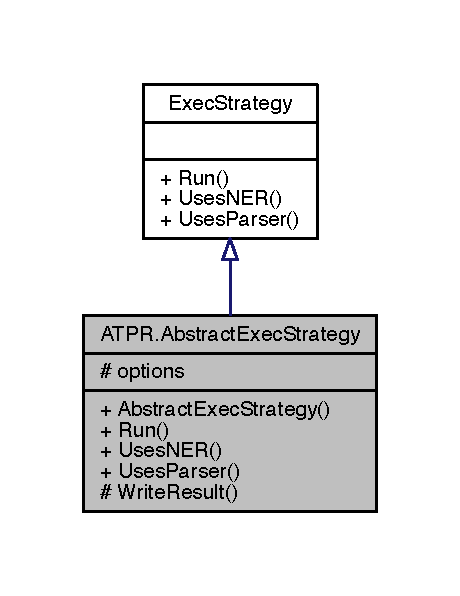
\includegraphics[width=221pt]{d8/dec/class_a_t_p_r_1_1_abstract_exec_strategy__inherit__graph}
\end{center}
\end{figure}


Collaboration diagram for A\+T\+P\+R.\+Abstract\+Exec\+Strategy\+:
\nopagebreak
\begin{figure}[H]
\begin{center}
\leavevmode
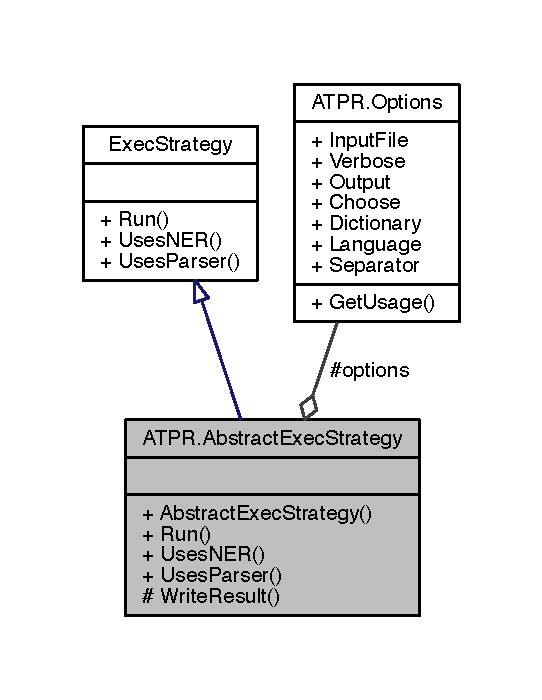
\includegraphics[width=260pt]{d1/dcb/class_a_t_p_r_1_1_abstract_exec_strategy__coll__graph}
\end{center}
\end{figure}
\subsection*{Public Member Functions}
\begin{DoxyCompactItemize}
\item 
\hypertarget{class_a_t_p_r_1_1_abstract_exec_strategy_a0fb3ff91dd3668e7bc5acea78d83598c}{}\label{class_a_t_p_r_1_1_abstract_exec_strategy_a0fb3ff91dd3668e7bc5acea78d83598c} 
{\bfseries Abstract\+Exec\+Strategy} (\hyperlink{class_a_t_p_r_1_1_options}{Options} options)
\item 
\hypertarget{class_a_t_p_r_1_1_abstract_exec_strategy_ac8fe75fd5a06c7fb01f64658dd3b35ae}{}\label{class_a_t_p_r_1_1_abstract_exec_strategy_ac8fe75fd5a06c7fb01f64658dd3b35ae} 
abstract void {\bfseries Run} ()
\item 
\hypertarget{class_a_t_p_r_1_1_abstract_exec_strategy_ab17073dc4fa6f287b5258d3f55fc1627}{}\label{class_a_t_p_r_1_1_abstract_exec_strategy_ab17073dc4fa6f287b5258d3f55fc1627} 
abstract bool {\bfseries Uses\+N\+ER} ()
\item 
\hypertarget{class_a_t_p_r_1_1_abstract_exec_strategy_a3d030a285e4dfe4256eefa335df3785b}{}\label{class_a_t_p_r_1_1_abstract_exec_strategy_a3d030a285e4dfe4256eefa335df3785b} 
abstract bool {\bfseries Uses\+Parser} ()
\end{DoxyCompactItemize}
\subsection*{Protected Member Functions}
\begin{DoxyCompactItemize}
\item 
void \hyperlink{class_a_t_p_r_1_1_abstract_exec_strategy_a5c7e5c801d158537a2f315bcb5ed91b8}{Write\+Result} (string result)
\begin{DoxyCompactList}\small\item\em Writes the run method result. \end{DoxyCompactList}\end{DoxyCompactItemize}
\subsection*{Protected Attributes}
\begin{DoxyCompactItemize}
\item 
\hypertarget{class_a_t_p_r_1_1_abstract_exec_strategy_aa6db79825edd147d1e98ffe52f18335f}{}\label{class_a_t_p_r_1_1_abstract_exec_strategy_aa6db79825edd147d1e98ffe52f18335f} 
\hyperlink{class_a_t_p_r_1_1_options}{Options} {\bfseries options}
\end{DoxyCompactItemize}


\subsection{Detailed Description}
Class that sets a common structure for all the strategies 



\subsection{Member Function Documentation}
\hypertarget{class_a_t_p_r_1_1_abstract_exec_strategy_a5c7e5c801d158537a2f315bcb5ed91b8}{}\label{class_a_t_p_r_1_1_abstract_exec_strategy_a5c7e5c801d158537a2f315bcb5ed91b8} 
\index{A\+T\+P\+R\+::\+Abstract\+Exec\+Strategy@{A\+T\+P\+R\+::\+Abstract\+Exec\+Strategy}!Write\+Result@{Write\+Result}}
\index{Write\+Result@{Write\+Result}!A\+T\+P\+R\+::\+Abstract\+Exec\+Strategy@{A\+T\+P\+R\+::\+Abstract\+Exec\+Strategy}}
\subsubsection{\texorpdfstring{Write\+Result()}{WriteResult()}}
{\footnotesize\ttfamily void A\+T\+P\+R.\+Abstract\+Exec\+Strategy.\+Write\+Result (\begin{DoxyParamCaption}\item[{string}]{result }\end{DoxyParamCaption})\hspace{0.3cm}{\ttfamily [inline]}, {\ttfamily [protected]}}



Writes the run method result. 


\begin{DoxyParams}{Parameters}
{\em result} & Result.\\
\hline
\end{DoxyParams}


The documentation for this class was generated from the following file\+:\begin{DoxyCompactItemize}
\item 
A\+T\+P\+R/Abstract\+Exec\+Strategy.\+cs\end{DoxyCompactItemize}

\hypertarget{class_a_t_p_r_n_e_r_1_1_c_r_f_classifiers}{}\section{A\+T\+P\+R\+N\+E\+R.\+C\+R\+F\+Classifiers Class Reference}
\label{class_a_t_p_r_n_e_r_1_1_c_r_f_classifiers}\index{A\+T\+P\+R\+N\+E\+R.\+C\+R\+F\+Classifiers@{A\+T\+P\+R\+N\+E\+R.\+C\+R\+F\+Classifiers}}


A multiton that stores Classifiers instances based on language  




Collaboration diagram for A\+T\+P\+R\+N\+E\+R.\+C\+R\+F\+Classifiers\+:
\nopagebreak
\begin{figure}[H]
\begin{center}
\leavevmode
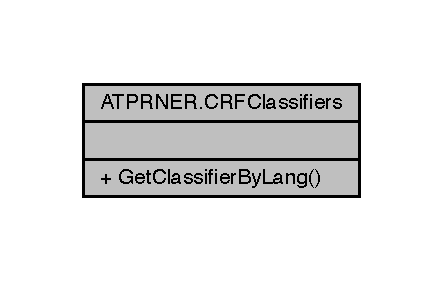
\includegraphics[width=212pt]{db/d99/class_a_t_p_r_n_e_r_1_1_c_r_f_classifiers__coll__graph}
\end{center}
\end{figure}
\subsection*{Static Public Member Functions}
\begin{DoxyCompactItemize}
\item 
\hypertarget{class_a_t_p_r_n_e_r_1_1_c_r_f_classifiers_a2f3b3220fd6ec5b56c3e6a6b79d81816}{}\label{class_a_t_p_r_n_e_r_1_1_c_r_f_classifiers_a2f3b3220fd6ec5b56c3e6a6b79d81816} 
static C\+R\+F\+Classifier {\bfseries Get\+Classifier\+By\+Lang} (string lang)
\end{DoxyCompactItemize}


\subsection{Detailed Description}
A multiton that stores Classifiers instances based on language 



The documentation for this class was generated from the following file\+:\begin{DoxyCompactItemize}
\item 
A\+T\+P\+R\+N\+E\+R/C\+R\+F\+Classifiers.\+cs\end{DoxyCompactItemize}

\hypertarget{class_a_t_p_r_n_e_r_1_1_dictionary_matcher}{}\section{A\+T\+P\+R\+N\+E\+R.\+Dictionary\+Matcher Class Reference}
\label{class_a_t_p_r_n_e_r_1_1_dictionary_matcher}\index{A\+T\+P\+R\+N\+E\+R.\+Dictionary\+Matcher@{A\+T\+P\+R\+N\+E\+R.\+Dictionary\+Matcher}}


Collaboration diagram for A\+T\+P\+R\+N\+E\+R.\+Dictionary\+Matcher\+:
\nopagebreak
\begin{figure}[H]
\begin{center}
\leavevmode
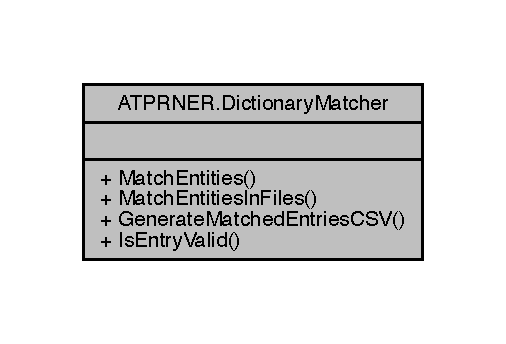
\includegraphics[width=226pt]{db/d42/class_a_t_p_r_n_e_r_1_1_dictionary_matcher__coll__graph}
\end{center}
\end{figure}
\subsection*{Static Public Member Functions}
\begin{DoxyCompactItemize}
\item 
static Dictionary$<$ string, \hyperlink{class_a_t_p_r_n_e_r_1_1_matched_entity}{Matched\+Entity} $>$ \hyperlink{class_a_t_p_r_n_e_r_1_1_dictionary_matcher_aa6fdeaf3a88c14b5ed8e4f452d1c3c17}{Match\+Entities} (List$<$ string\mbox{[}$\,$\mbox{]}$>$ text\+Entities, List$<$ string $>$ dict\+Entities)
\begin{DoxyCompactList}\small\item\em Matchs the text entities with the dictionary entities. \end{DoxyCompactList}\item 
static void \hyperlink{class_a_t_p_r_n_e_r_1_1_dictionary_matcher_a6fc36cbd0e0df420c2aaafa389ae7b61}{Match\+Entities\+In\+Files} (string input\+Path, string dic\+Path, Text\+Writer output, char sep)
\begin{DoxyCompactList}\small\item\em Writes to the output stream a csv with the match results against the dictionary \end{DoxyCompactList}\end{DoxyCompactItemize}


\subsection{Member Function Documentation}
\hypertarget{class_a_t_p_r_n_e_r_1_1_dictionary_matcher_aa6fdeaf3a88c14b5ed8e4f452d1c3c17}{}\label{class_a_t_p_r_n_e_r_1_1_dictionary_matcher_aa6fdeaf3a88c14b5ed8e4f452d1c3c17} 
\index{A\+T\+P\+R\+N\+E\+R\+::\+Dictionary\+Matcher@{A\+T\+P\+R\+N\+E\+R\+::\+Dictionary\+Matcher}!Match\+Entities@{Match\+Entities}}
\index{Match\+Entities@{Match\+Entities}!A\+T\+P\+R\+N\+E\+R\+::\+Dictionary\+Matcher@{A\+T\+P\+R\+N\+E\+R\+::\+Dictionary\+Matcher}}
\subsubsection{\texorpdfstring{Match\+Entities()}{MatchEntities()}}
{\footnotesize\ttfamily static Dictionary$<$string, \hyperlink{class_a_t_p_r_n_e_r_1_1_matched_entity}{Matched\+Entity}$>$ A\+T\+P\+R\+N\+E\+R.\+Dictionary\+Matcher.\+Match\+Entities (\begin{DoxyParamCaption}\item[{List$<$ string\mbox{[}$\,$\mbox{]}$>$}]{text\+Entities,  }\item[{List$<$ string $>$}]{dict\+Entities }\end{DoxyParamCaption})\hspace{0.3cm}{\ttfamily [inline]}, {\ttfamily [static]}}



Matchs the text entities with the dictionary entities. 

\begin{DoxyReturn}{Returns}
The entities.
\end{DoxyReturn}

\begin{DoxyParams}{Parameters}
{\em text\+Entities} & Text entities.\\
\hline
{\em dict\+Entities} & Dict entities.\\
\hline
\end{DoxyParams}
Here is the caller graph for this function\+:
\nopagebreak
\begin{figure}[H]
\begin{center}
\leavevmode
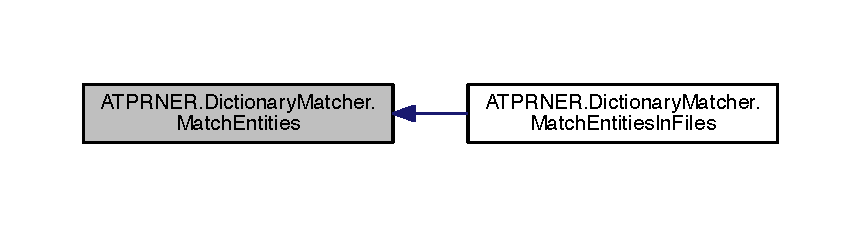
\includegraphics[width=350pt]{d0/d6a/class_a_t_p_r_n_e_r_1_1_dictionary_matcher_aa6fdeaf3a88c14b5ed8e4f452d1c3c17_icgraph}
\end{center}
\end{figure}
\hypertarget{class_a_t_p_r_n_e_r_1_1_dictionary_matcher_a6fc36cbd0e0df420c2aaafa389ae7b61}{}\label{class_a_t_p_r_n_e_r_1_1_dictionary_matcher_a6fc36cbd0e0df420c2aaafa389ae7b61} 
\index{A\+T\+P\+R\+N\+E\+R\+::\+Dictionary\+Matcher@{A\+T\+P\+R\+N\+E\+R\+::\+Dictionary\+Matcher}!Match\+Entities\+In\+Files@{Match\+Entities\+In\+Files}}
\index{Match\+Entities\+In\+Files@{Match\+Entities\+In\+Files}!A\+T\+P\+R\+N\+E\+R\+::\+Dictionary\+Matcher@{A\+T\+P\+R\+N\+E\+R\+::\+Dictionary\+Matcher}}
\subsubsection{\texorpdfstring{Match\+Entities\+In\+Files()}{MatchEntitiesInFiles()}}
{\footnotesize\ttfamily static void A\+T\+P\+R\+N\+E\+R.\+Dictionary\+Matcher.\+Match\+Entities\+In\+Files (\begin{DoxyParamCaption}\item[{string}]{input\+Path,  }\item[{string}]{dic\+Path,  }\item[{Text\+Writer}]{output,  }\item[{char}]{sep }\end{DoxyParamCaption})\hspace{0.3cm}{\ttfamily [inline]}, {\ttfamily [static]}}



Writes to the output stream a csv with the match results against the dictionary 


\begin{DoxyParams}{Parameters}
{\em input\+Path} & Files path.\\
\hline
{\em dic\+Path} & Dictionary path.\\
\hline
{\em output} & Output stream.\\
\hline
\end{DoxyParams}
Here is the call graph for this function\+:
\nopagebreak
\begin{figure}[H]
\begin{center}
\leavevmode
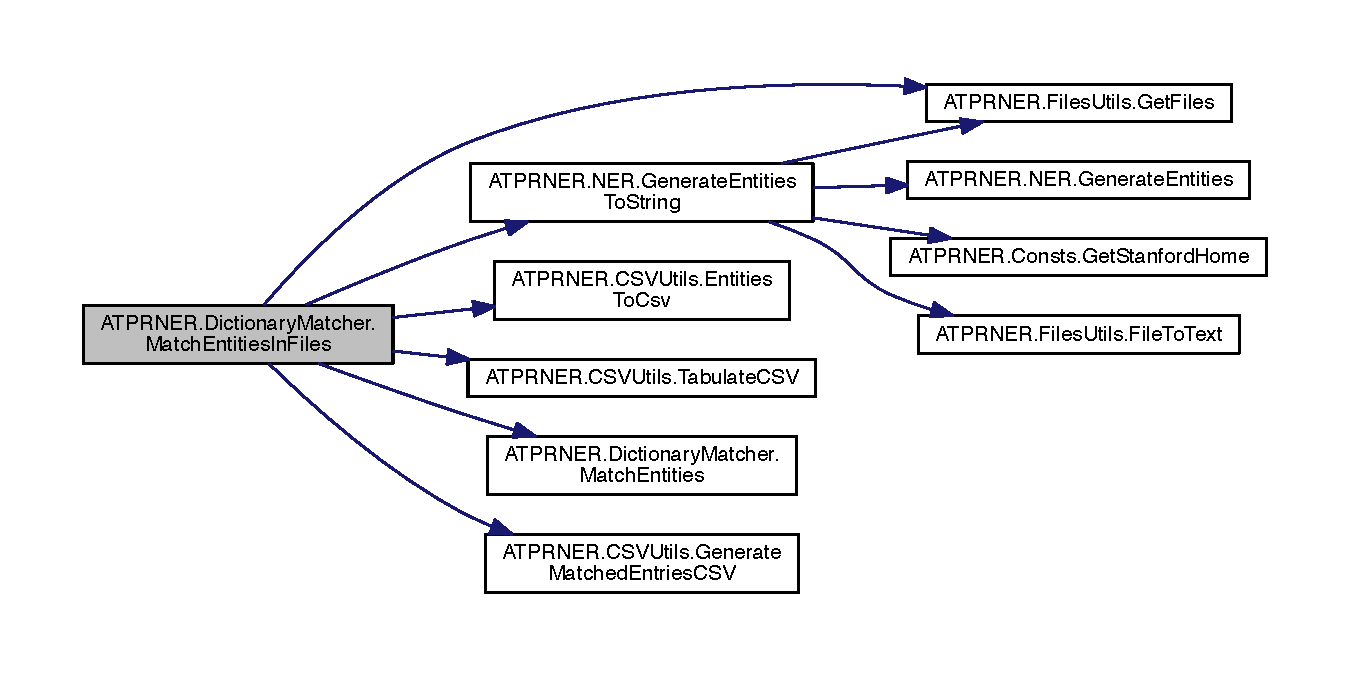
\includegraphics[width=350pt]{d0/d6a/class_a_t_p_r_n_e_r_1_1_dictionary_matcher_a6fc36cbd0e0df420c2aaafa389ae7b61_cgraph}
\end{center}
\end{figure}
Here is the caller graph for this function\+:
\nopagebreak
\begin{figure}[H]
\begin{center}
\leavevmode
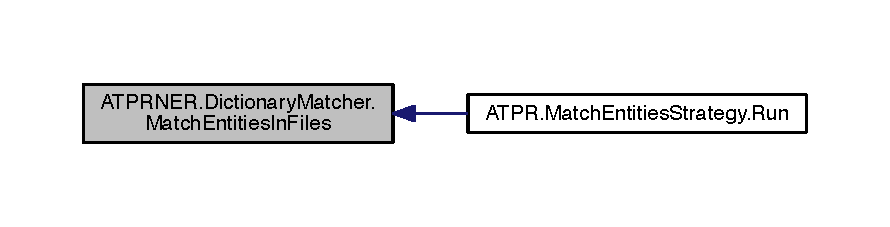
\includegraphics[width=350pt]{d0/d6a/class_a_t_p_r_n_e_r_1_1_dictionary_matcher_a6fc36cbd0e0df420c2aaafa389ae7b61_icgraph}
\end{center}
\end{figure}


The documentation for this class was generated from the following file\+:\begin{DoxyCompactItemize}
\item 
A\+T\+P\+R\+N\+E\+R/Dictionary\+Matcher.\+cs\end{DoxyCompactItemize}

\hypertarget{interface_a_t_p_r_1_1_exec_strategy}{}\section{A\+T\+P\+R.\+Exec\+Strategy Interface Reference}
\label{interface_a_t_p_r_1_1_exec_strategy}\index{A\+T\+P\+R.\+Exec\+Strategy@{A\+T\+P\+R.\+Exec\+Strategy}}


Base interface for strategy classes  




Inheritance diagram for A\+T\+P\+R.\+Exec\+Strategy\+:
\nopagebreak
\begin{figure}[H]
\begin{center}
\leavevmode
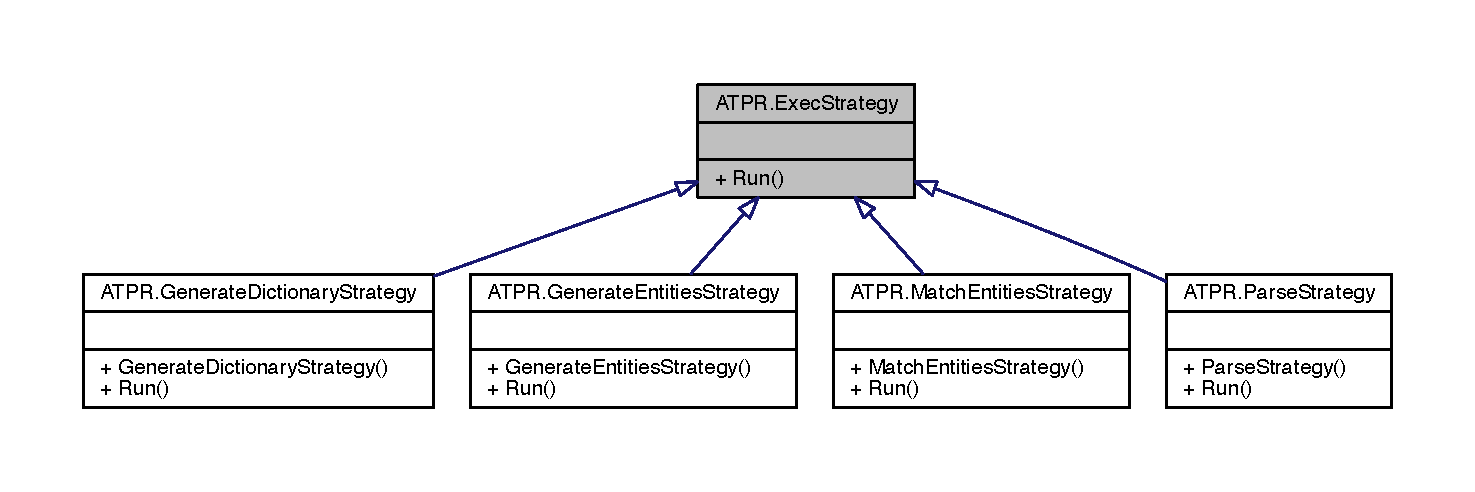
\includegraphics[width=221pt]{d2/d3b/interface_a_t_p_r_1_1_exec_strategy__inherit__graph}
\end{center}
\end{figure}


Collaboration diagram for A\+T\+P\+R.\+Exec\+Strategy\+:
\nopagebreak
\begin{figure}[H]
\begin{center}
\leavevmode
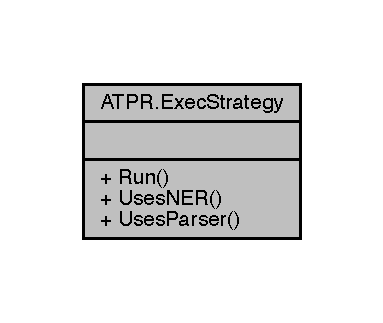
\includegraphics[width=184pt]{d9/db3/interface_a_t_p_r_1_1_exec_strategy__coll__graph}
\end{center}
\end{figure}
\subsection*{Public Member Functions}
\begin{DoxyCompactItemize}
\item 
\hypertarget{interface_a_t_p_r_1_1_exec_strategy_adcd52fae2702ce31b645ec8d149c0e51}{}\label{interface_a_t_p_r_1_1_exec_strategy_adcd52fae2702ce31b645ec8d149c0e51} 
void {\bfseries Run} ()
\item 
\hypertarget{interface_a_t_p_r_1_1_exec_strategy_acd32c810cb2247e7b058520cce7ed3cb}{}\label{interface_a_t_p_r_1_1_exec_strategy_acd32c810cb2247e7b058520cce7ed3cb} 
bool {\bfseries Uses\+N\+ER} ()
\item 
\hypertarget{interface_a_t_p_r_1_1_exec_strategy_a04e0c2d18b63468c4255c08182620726}{}\label{interface_a_t_p_r_1_1_exec_strategy_a04e0c2d18b63468c4255c08182620726} 
bool {\bfseries Uses\+Parser} ()
\end{DoxyCompactItemize}


\subsection{Detailed Description}
Base interface for strategy classes 



The documentation for this interface was generated from the following file\+:\begin{DoxyCompactItemize}
\item 
A\+T\+P\+R/Exec\+Strategy.\+cs\end{DoxyCompactItemize}

\hypertarget{interface_a_t_p_r_1_1_i_match_iterator}{}\section{A\+T\+P\+R.\+I\+Match\+Iterator Interface Reference}
\label{interface_a_t_p_r_1_1_i_match_iterator}\index{A\+T\+P\+R.\+I\+Match\+Iterator@{A\+T\+P\+R.\+I\+Match\+Iterator}}


Interface for iterating matches.  




Inheritance diagram for A\+T\+P\+R.\+I\+Match\+Iterator\+:
\nopagebreak
\begin{figure}[H]
\begin{center}
\leavevmode
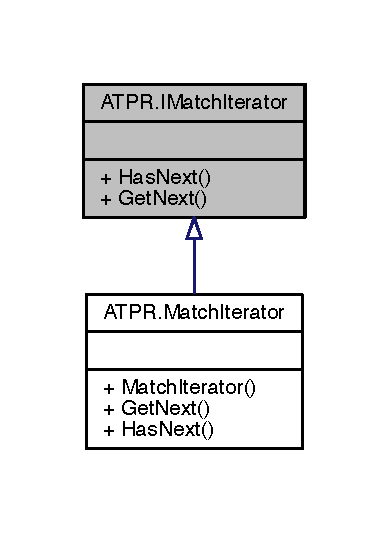
\includegraphics[width=186pt]{d9/d31/interface_a_t_p_r_1_1_i_match_iterator__inherit__graph}
\end{center}
\end{figure}


Collaboration diagram for A\+T\+P\+R.\+I\+Match\+Iterator\+:
\nopagebreak
\begin{figure}[H]
\begin{center}
\leavevmode
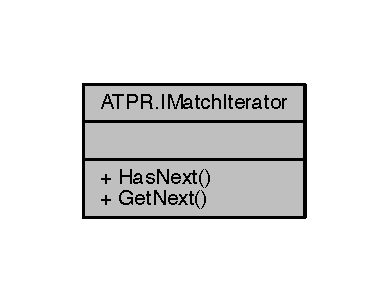
\includegraphics[width=186pt]{d2/df5/interface_a_t_p_r_1_1_i_match_iterator__coll__graph}
\end{center}
\end{figure}
\subsection*{Public Member Functions}
\begin{DoxyCompactItemize}
\item 
\hypertarget{interface_a_t_p_r_1_1_i_match_iterator_a806d473502d3d29370b2f72a3bbc3b00}{}\label{interface_a_t_p_r_1_1_i_match_iterator_a806d473502d3d29370b2f72a3bbc3b00} 
bool {\bfseries Has\+Next} ()
\item 
\hypertarget{interface_a_t_p_r_1_1_i_match_iterator_aef36e63440805a95c95d68480ba189a0}{}\label{interface_a_t_p_r_1_1_i_match_iterator_aef36e63440805a95c95d68480ba189a0} 
\hyperlink{class_a_t_p_r_1_1_match}{Match} {\bfseries Get\+Next} ()
\end{DoxyCompactItemize}


\subsection{Detailed Description}
Interface for iterating matches. 



The documentation for this interface was generated from the following file\+:\begin{DoxyCompactItemize}
\item 
A\+T\+P\+R/I\+Match\+Iterator.\+cs\end{DoxyCompactItemize}

\hypertarget{class_a_t_p_r_1_1_main_class}{}\section{A\+T\+P\+R.\+Main\+Class Class Reference}
\label{class_a_t_p_r_1_1_main_class}\index{A\+T\+P\+R.\+Main\+Class@{A\+T\+P\+R.\+Main\+Class}}


The documentation for this class was generated from the following file\+:\begin{DoxyCompactItemize}
\item 
A\+T\+P\+R/Program.\+cs\end{DoxyCompactItemize}

\hypertarget{class_a_t_p_r_1_1_match}{}\section{A\+T\+P\+R.\+Match Class Reference}
\label{class_a_t_p_r_1_1_match}\index{A\+T\+P\+R.\+Match@{A\+T\+P\+R.\+Match}}


Stores a match with the text of the source file  




Collaboration diagram for A\+T\+P\+R.\+Match\+:
\nopagebreak
\begin{figure}[H]
\begin{center}
\leavevmode
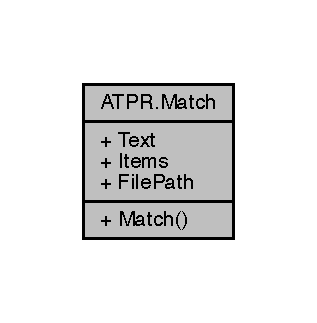
\includegraphics[width=152pt]{d4/d82/class_a_t_p_r_1_1_match__coll__graph}
\end{center}
\end{figure}
\subsection*{Public Member Functions}
\begin{DoxyCompactItemize}
\item 
\hypertarget{class_a_t_p_r_1_1_match_a306eee0d1885fb716091fcd7ce99515d}{}\label{class_a_t_p_r_1_1_match_a306eee0d1885fb716091fcd7ce99515d} 
{\bfseries Match} (string file\+Path, List$<$ string\mbox{[}$\,$\mbox{]}$>$ items)
\end{DoxyCompactItemize}
\subsection*{Properties}
\begin{DoxyCompactItemize}
\item 
\hypertarget{class_a_t_p_r_1_1_match_a2b0e5fd5ce30a4c94427f1625fc18277}{}\label{class_a_t_p_r_1_1_match_a2b0e5fd5ce30a4c94427f1625fc18277} 
string {\bfseries Text}\hspace{0.3cm}{\ttfamily  \mbox{[}get\mbox{]}}
\item 
\hypertarget{class_a_t_p_r_1_1_match_ab2c45325967b080e1d391bcdb14b8759}{}\label{class_a_t_p_r_1_1_match_ab2c45325967b080e1d391bcdb14b8759} 
List$<$ string\mbox{[}$\,$\mbox{]}$>$ {\bfseries Items}\hspace{0.3cm}{\ttfamily  \mbox{[}get\mbox{]}}
\item 
\hypertarget{class_a_t_p_r_1_1_match_a22f9ef303775cd648e278fe57a098f22}{}\label{class_a_t_p_r_1_1_match_a22f9ef303775cd648e278fe57a098f22} 
string {\bfseries File\+Path}\hspace{0.3cm}{\ttfamily  \mbox{[}get\mbox{]}}
\end{DoxyCompactItemize}


\subsection{Detailed Description}
Stores a match with the text of the source file 



The documentation for this class was generated from the following file\+:\begin{DoxyCompactItemize}
\item 
A\+T\+P\+R/Match.\+cs\end{DoxyCompactItemize}

\hypertarget{class_a_t_p_r_n_e_r_1_1_matched_entity}{}\section{A\+T\+P\+R\+N\+E\+R.\+Matched\+Entity Class Reference}
\label{class_a_t_p_r_n_e_r_1_1_matched_entity}\index{A\+T\+P\+R\+N\+E\+R.\+Matched\+Entity@{A\+T\+P\+R\+N\+E\+R.\+Matched\+Entity}}


Represents the matched entitiy with the information needed.  




Collaboration diagram for A\+T\+P\+R\+N\+E\+R.\+Matched\+Entity\+:\nopagebreak
\begin{figure}[H]
\begin{center}
\leavevmode
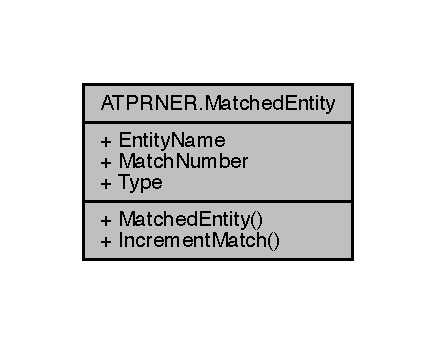
\includegraphics[width=209pt]{d6/dd7/class_a_t_p_r_n_e_r_1_1_matched_entity__coll__graph}
\end{center}
\end{figure}
\subsection*{Public Member Functions}
\begin{DoxyCompactItemize}
\item 
\hyperlink{class_a_t_p_r_n_e_r_1_1_matched_entity_a5737ccd3008395ca92559e0b1b1f3e73}{Matched\+Entity} (String entity\+Name, String type)
\begin{DoxyCompactList}\small\item\em Initializes a new instance of the \hyperlink{class_a_t_p_r_n_e_r_1_1_matched_entity}{A\+T\+P\+R\+N\+E\+R.\+Matched\+Entity} class. \end{DoxyCompactList}\item 
void \hyperlink{class_a_t_p_r_n_e_r_1_1_matched_entity_ae6fa09ea42c0787d4279ceb5076c5f14}{Increment\+Match} ()
\begin{DoxyCompactList}\small\item\em Increments the match number one unity. \end{DoxyCompactList}\end{DoxyCompactItemize}
\subsection*{Properties}
\begin{DoxyCompactItemize}
\item 
String \hyperlink{class_a_t_p_r_n_e_r_1_1_matched_entity_a42a05257a07b5d089ac070b1d9e5461a}{Entity\+Name}\hspace{0.3cm}{\ttfamily  \mbox{[}get, set\mbox{]}}
\begin{DoxyCompactList}\small\item\em Gets or sets the name of the entity. \end{DoxyCompactList}\item 
int \hyperlink{class_a_t_p_r_n_e_r_1_1_matched_entity_ad6ca936e2b54158984f7d7d3753d1490}{Match\+Number}\hspace{0.3cm}{\ttfamily  \mbox{[}get, set\mbox{]}}
\begin{DoxyCompactList}\small\item\em Gets or sets the match number. \end{DoxyCompactList}\item 
String \hyperlink{class_a_t_p_r_n_e_r_1_1_matched_entity_af7d651ec944931f14c26eedffc4150de}{Type}\hspace{0.3cm}{\ttfamily  \mbox{[}get, set\mbox{]}}
\begin{DoxyCompactList}\small\item\em Gets or sets the type. \end{DoxyCompactList}\end{DoxyCompactItemize}


\subsection{Detailed Description}
Represents the matched entitiy with the information needed. 



\subsection{Constructor \& Destructor Documentation}
\hypertarget{class_a_t_p_r_n_e_r_1_1_matched_entity_a5737ccd3008395ca92559e0b1b1f3e73}{}\label{class_a_t_p_r_n_e_r_1_1_matched_entity_a5737ccd3008395ca92559e0b1b1f3e73} 
\index{A\+T\+P\+R\+N\+E\+R\+::\+Matched\+Entity@{A\+T\+P\+R\+N\+E\+R\+::\+Matched\+Entity}!Matched\+Entity@{Matched\+Entity}}
\index{Matched\+Entity@{Matched\+Entity}!A\+T\+P\+R\+N\+E\+R\+::\+Matched\+Entity@{A\+T\+P\+R\+N\+E\+R\+::\+Matched\+Entity}}
\subsubsection{\texorpdfstring{Matched\+Entity()}{MatchedEntity()}}
{\footnotesize\ttfamily A\+T\+P\+R\+N\+E\+R.\+Matched\+Entity.\+Matched\+Entity (\begin{DoxyParamCaption}\item[{String}]{entity\+Name,  }\item[{String}]{type }\end{DoxyParamCaption})\hspace{0.3cm}{\ttfamily [inline]}}



Initializes a new instance of the \hyperlink{class_a_t_p_r_n_e_r_1_1_matched_entity}{A\+T\+P\+R\+N\+E\+R.\+Matched\+Entity} class. 


\begin{DoxyParams}{Parameters}
{\em entity\+Name} & Entity name.\\
\hline
\end{DoxyParams}


\subsection{Member Function Documentation}
\hypertarget{class_a_t_p_r_n_e_r_1_1_matched_entity_ae6fa09ea42c0787d4279ceb5076c5f14}{}\label{class_a_t_p_r_n_e_r_1_1_matched_entity_ae6fa09ea42c0787d4279ceb5076c5f14} 
\index{A\+T\+P\+R\+N\+E\+R\+::\+Matched\+Entity@{A\+T\+P\+R\+N\+E\+R\+::\+Matched\+Entity}!Increment\+Match@{Increment\+Match}}
\index{Increment\+Match@{Increment\+Match}!A\+T\+P\+R\+N\+E\+R\+::\+Matched\+Entity@{A\+T\+P\+R\+N\+E\+R\+::\+Matched\+Entity}}
\subsubsection{\texorpdfstring{Increment\+Match()}{IncrementMatch()}}
{\footnotesize\ttfamily void A\+T\+P\+R\+N\+E\+R.\+Matched\+Entity.\+Increment\+Match (\begin{DoxyParamCaption}{ }\end{DoxyParamCaption})\hspace{0.3cm}{\ttfamily [inline]}}



Increments the match number one unity. 



\subsection{Property Documentation}
\hypertarget{class_a_t_p_r_n_e_r_1_1_matched_entity_a42a05257a07b5d089ac070b1d9e5461a}{}\label{class_a_t_p_r_n_e_r_1_1_matched_entity_a42a05257a07b5d089ac070b1d9e5461a} 
\index{A\+T\+P\+R\+N\+E\+R\+::\+Matched\+Entity@{A\+T\+P\+R\+N\+E\+R\+::\+Matched\+Entity}!Entity\+Name@{Entity\+Name}}
\index{Entity\+Name@{Entity\+Name}!A\+T\+P\+R\+N\+E\+R\+::\+Matched\+Entity@{A\+T\+P\+R\+N\+E\+R\+::\+Matched\+Entity}}
\subsubsection{\texorpdfstring{Entity\+Name}{EntityName}}
{\footnotesize\ttfamily String A\+T\+P\+R\+N\+E\+R.\+Matched\+Entity.\+Entity\+Name\hspace{0.3cm}{\ttfamily [get]}, {\ttfamily [set]}}



Gets or sets the name of the entity. 

The name of the entity.\hypertarget{class_a_t_p_r_n_e_r_1_1_matched_entity_ad6ca936e2b54158984f7d7d3753d1490}{}\label{class_a_t_p_r_n_e_r_1_1_matched_entity_ad6ca936e2b54158984f7d7d3753d1490} 
\index{A\+T\+P\+R\+N\+E\+R\+::\+Matched\+Entity@{A\+T\+P\+R\+N\+E\+R\+::\+Matched\+Entity}!Match\+Number@{Match\+Number}}
\index{Match\+Number@{Match\+Number}!A\+T\+P\+R\+N\+E\+R\+::\+Matched\+Entity@{A\+T\+P\+R\+N\+E\+R\+::\+Matched\+Entity}}
\subsubsection{\texorpdfstring{Match\+Number}{MatchNumber}}
{\footnotesize\ttfamily int A\+T\+P\+R\+N\+E\+R.\+Matched\+Entity.\+Match\+Number\hspace{0.3cm}{\ttfamily [get]}, {\ttfamily [set]}}



Gets or sets the match number. 

The match number.\hypertarget{class_a_t_p_r_n_e_r_1_1_matched_entity_af7d651ec944931f14c26eedffc4150de}{}\label{class_a_t_p_r_n_e_r_1_1_matched_entity_af7d651ec944931f14c26eedffc4150de} 
\index{A\+T\+P\+R\+N\+E\+R\+::\+Matched\+Entity@{A\+T\+P\+R\+N\+E\+R\+::\+Matched\+Entity}!Type@{Type}}
\index{Type@{Type}!A\+T\+P\+R\+N\+E\+R\+::\+Matched\+Entity@{A\+T\+P\+R\+N\+E\+R\+::\+Matched\+Entity}}
\subsubsection{\texorpdfstring{Type}{Type}}
{\footnotesize\ttfamily String A\+T\+P\+R\+N\+E\+R.\+Matched\+Entity.\+Type\hspace{0.3cm}{\ttfamily [get]}, {\ttfamily [set]}}



Gets or sets the type. 

The type.

The documentation for this class was generated from the following file\+:\begin{DoxyCompactItemize}
\item 
A\+T\+P\+R\+N\+E\+R/Matched\+Entity.\+cs\end{DoxyCompactItemize}

\hypertarget{class_a_t_p_r_1_1_match_iterator}{}\section{A\+T\+P\+R.\+Match\+Iterator Class Reference}
\label{class_a_t_p_r_1_1_match_iterator}\index{A\+T\+P\+R.\+Match\+Iterator@{A\+T\+P\+R.\+Match\+Iterator}}


Iterates over the matched entries  




Inheritance diagram for A\+T\+P\+R.\+Match\+Iterator\+:
\nopagebreak
\begin{figure}[H]
\begin{center}
\leavevmode
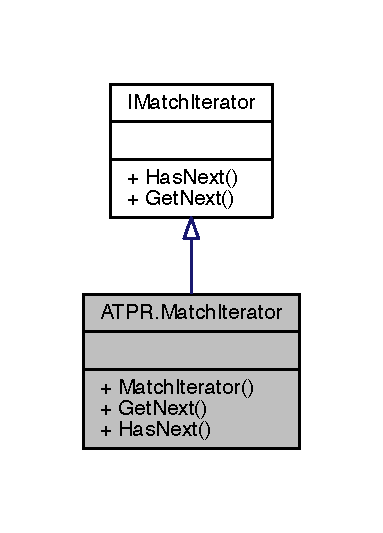
\includegraphics[width=184pt]{d2/d37/class_a_t_p_r_1_1_match_iterator__inherit__graph}
\end{center}
\end{figure}


Collaboration diagram for A\+T\+P\+R.\+Match\+Iterator\+:
\nopagebreak
\begin{figure}[H]
\begin{center}
\leavevmode
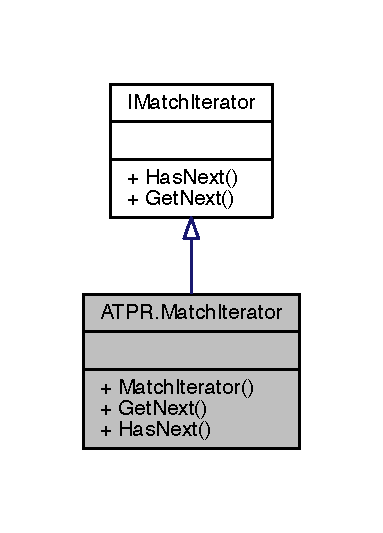
\includegraphics[width=184pt]{dd/dcf/class_a_t_p_r_1_1_match_iterator__coll__graph}
\end{center}
\end{figure}
\subsection*{Public Member Functions}
\begin{DoxyCompactItemize}
\item 
\hypertarget{class_a_t_p_r_1_1_match_iterator_a6baba4b1475c60b1b89609d517c4ba1b}{}\label{class_a_t_p_r_1_1_match_iterator_a6baba4b1475c60b1b89609d517c4ba1b} 
{\bfseries Match\+Iterator} (List$<$ string\mbox{[}$\,$\mbox{]}$>$ matches)
\item 
\hyperlink{class_a_t_p_r_1_1_match}{Match} \hyperlink{class_a_t_p_r_1_1_match_iterator_a72658237a15b16825e73b72d3d8ed4e2}{Get\+Next} ()
\begin{DoxyCompactList}\small\item\em Returns the next matches grouped by source file \end{DoxyCompactList}\item 
bool \hyperlink{class_a_t_p_r_1_1_match_iterator_a65b39ac2d89a16934d81a8992767d3e9}{Has\+Next} ()
\begin{DoxyCompactList}\small\item\em Returns true if there are more matches \end{DoxyCompactList}\end{DoxyCompactItemize}


\subsection{Detailed Description}
Iterates over the matched entries 



\subsection{Member Function Documentation}
\hypertarget{class_a_t_p_r_1_1_match_iterator_a72658237a15b16825e73b72d3d8ed4e2}{}\label{class_a_t_p_r_1_1_match_iterator_a72658237a15b16825e73b72d3d8ed4e2} 
\index{A\+T\+P\+R\+::\+Match\+Iterator@{A\+T\+P\+R\+::\+Match\+Iterator}!Get\+Next@{Get\+Next}}
\index{Get\+Next@{Get\+Next}!A\+T\+P\+R\+::\+Match\+Iterator@{A\+T\+P\+R\+::\+Match\+Iterator}}
\subsubsection{\texorpdfstring{Get\+Next()}{GetNext()}}
{\footnotesize\ttfamily \hyperlink{class_a_t_p_r_1_1_match}{Match} A\+T\+P\+R.\+Match\+Iterator.\+Get\+Next (\begin{DoxyParamCaption}{ }\end{DoxyParamCaption})\hspace{0.3cm}{\ttfamily [inline]}}



Returns the next matches grouped by source file 

\begin{DoxyReturn}{Returns}
The next.
\end{DoxyReturn}


Implements \hyperlink{interface_a_t_p_r_1_1_i_match_iterator}{A\+T\+P\+R.\+I\+Match\+Iterator}.

Here is the call graph for this function\+:
\nopagebreak
\begin{figure}[H]
\begin{center}
\leavevmode
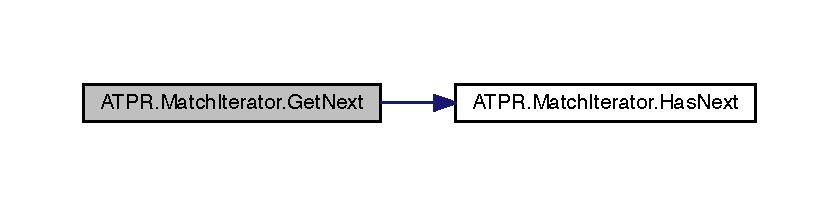
\includegraphics[width=350pt]{d1/d21/class_a_t_p_r_1_1_match_iterator_a72658237a15b16825e73b72d3d8ed4e2_cgraph}
\end{center}
\end{figure}
\hypertarget{class_a_t_p_r_1_1_match_iterator_a65b39ac2d89a16934d81a8992767d3e9}{}\label{class_a_t_p_r_1_1_match_iterator_a65b39ac2d89a16934d81a8992767d3e9} 
\index{A\+T\+P\+R\+::\+Match\+Iterator@{A\+T\+P\+R\+::\+Match\+Iterator}!Has\+Next@{Has\+Next}}
\index{Has\+Next@{Has\+Next}!A\+T\+P\+R\+::\+Match\+Iterator@{A\+T\+P\+R\+::\+Match\+Iterator}}
\subsubsection{\texorpdfstring{Has\+Next()}{HasNext()}}
{\footnotesize\ttfamily bool A\+T\+P\+R.\+Match\+Iterator.\+Has\+Next (\begin{DoxyParamCaption}{ }\end{DoxyParamCaption})\hspace{0.3cm}{\ttfamily [inline]}}



Returns true if there are more matches 

\begin{DoxyReturn}{Returns}
{\ttfamily true}, if there are more, {\ttfamily false} otherwise.
\end{DoxyReturn}


Implements \hyperlink{interface_a_t_p_r_1_1_i_match_iterator}{A\+T\+P\+R.\+I\+Match\+Iterator}.

Here is the caller graph for this function\+:
\nopagebreak
\begin{figure}[H]
\begin{center}
\leavevmode
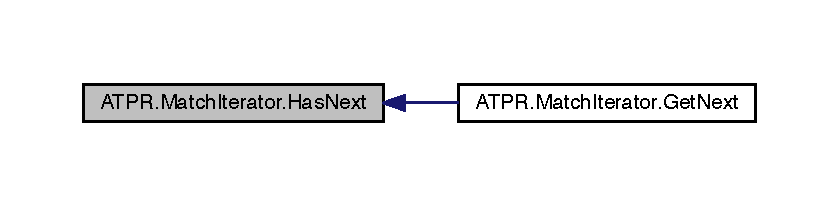
\includegraphics[width=350pt]{d1/d21/class_a_t_p_r_1_1_match_iterator_a65b39ac2d89a16934d81a8992767d3e9_icgraph}
\end{center}
\end{figure}


The documentation for this class was generated from the following file\+:\begin{DoxyCompactItemize}
\item 
A\+T\+P\+R/Match\+Iterator.\+cs\end{DoxyCompactItemize}

\hypertarget{class_a_t_p_r_1_1_options}{}\section{A\+T\+P\+R.\+Options Class Reference}
\label{class_a_t_p_r_1_1_options}\index{A\+T\+P\+R.\+Options@{A\+T\+P\+R.\+Options}}


Argument parse options.  




Collaboration diagram for A\+T\+P\+R.\+Options\+:
\nopagebreak
\begin{figure}[H]
\begin{center}
\leavevmode
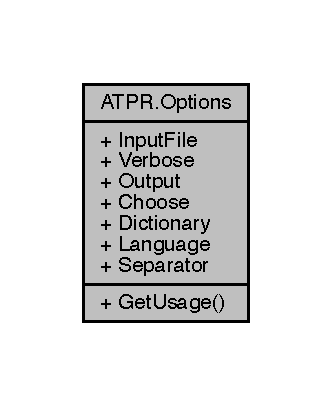
\includegraphics[width=159pt]{d4/dc3/class_a_t_p_r_1_1_options__coll__graph}
\end{center}
\end{figure}
\subsection*{Public Member Functions}
\begin{DoxyCompactItemize}
\item 
\hypertarget{class_a_t_p_r_1_1_options_a92883d4a7564f235412e41e6724c32b2}{}\label{class_a_t_p_r_1_1_options_a92883d4a7564f235412e41e6724c32b2} 
string {\bfseries Get\+Usage} ()
\end{DoxyCompactItemize}
\subsection*{Properties}
\begin{DoxyCompactItemize}
\item 
\hypertarget{class_a_t_p_r_1_1_options_ac0a2d51d6f7ef81700651d3951f51e4f}{}\label{class_a_t_p_r_1_1_options_ac0a2d51d6f7ef81700651d3951f51e4f} 
string {\bfseries Input\+File}\hspace{0.3cm}{\ttfamily  \mbox{[}get, set\mbox{]}}
\item 
\hypertarget{class_a_t_p_r_1_1_options_a8cb44ee6dbab360a3d9412626c2fa2d9}{}\label{class_a_t_p_r_1_1_options_a8cb44ee6dbab360a3d9412626c2fa2d9} 
bool {\bfseries Verbose}\hspace{0.3cm}{\ttfamily  \mbox{[}get, set\mbox{]}}
\item 
\hypertarget{class_a_t_p_r_1_1_options_a933d1d83e25d63f9b006c48efe3b4fd1}{}\label{class_a_t_p_r_1_1_options_a933d1d83e25d63f9b006c48efe3b4fd1} 
string {\bfseries Output}\hspace{0.3cm}{\ttfamily  \mbox{[}get, set\mbox{]}}
\item 
\hypertarget{class_a_t_p_r_1_1_options_a2b57c8aeea07cb4359ca235c24cd6cfe}{}\label{class_a_t_p_r_1_1_options_a2b57c8aeea07cb4359ca235c24cd6cfe} 
string {\bfseries Choose}\hspace{0.3cm}{\ttfamily  \mbox{[}get, set\mbox{]}}
\item 
\hypertarget{class_a_t_p_r_1_1_options_a5187c31694e58eb5cd7464b3c1f5eacc}{}\label{class_a_t_p_r_1_1_options_a5187c31694e58eb5cd7464b3c1f5eacc} 
string {\bfseries Dictionary}\hspace{0.3cm}{\ttfamily  \mbox{[}get, set\mbox{]}}
\item 
\hypertarget{class_a_t_p_r_1_1_options_af1d36310babdada573488c4795ee9a92}{}\label{class_a_t_p_r_1_1_options_af1d36310babdada573488c4795ee9a92} 
string {\bfseries Language}\hspace{0.3cm}{\ttfamily  \mbox{[}get, set\mbox{]}}
\item 
\hypertarget{class_a_t_p_r_1_1_options_ab40c002e4eeede247c68606cb3481a0f}{}\label{class_a_t_p_r_1_1_options_ab40c002e4eeede247c68606cb3481a0f} 
char {\bfseries Separator}\hspace{0.3cm}{\ttfamily  \mbox{[}get, set\mbox{]}}
\end{DoxyCompactItemize}


\subsection{Detailed Description}
Argument parse options. 



The documentation for this class was generated from the following file\+:\begin{DoxyCompactItemize}
\item 
A\+T\+P\+R/Options.\+cs\end{DoxyCompactItemize}

\hypertarget{class_a_t_p_r_parser_1_1_parser}{}\section{A\+T\+P\+R\+Parser.\+Parser Class Reference}
\label{class_a_t_p_r_parser_1_1_parser}\index{A\+T\+P\+R\+Parser.\+Parser@{A\+T\+P\+R\+Parser.\+Parser}}


\hyperlink{class_a_t_p_r_parser_1_1_parser}{Parser} Extracts the sentences where entities appear and parse it generating his syntactic analysis.  




Collaboration diagram for A\+T\+P\+R\+Parser.\+Parser\+:
\nopagebreak
\begin{figure}[H]
\begin{center}
\leavevmode
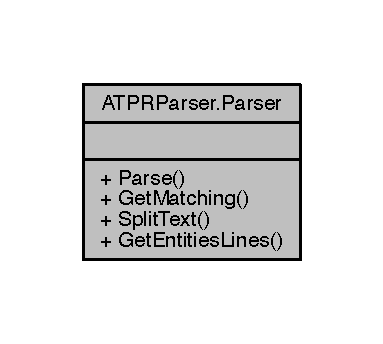
\includegraphics[width=184pt]{de/d41/class_a_t_p_r_parser_1_1_parser__coll__graph}
\end{center}
\end{figure}
\subsection*{Static Public Member Functions}
\begin{DoxyCompactItemize}
\item 
static List$<$ string\mbox{[}$\,$\mbox{]}$>$ \hyperlink{class_a_t_p_r_parser_1_1_parser_a4d0782c4136575c1b9a33102be225ea1}{Parse} (string text, string entity, string orig\+File, string language)
\begin{DoxyCompactList}\small\item\em Parse the document searching for sentences where the entity found. Returns a csv line with the file, the entity the sentence and the sintax analisis of the sentences \end{DoxyCompactList}\item 
static List$<$ String\mbox{[}$\,$\mbox{]}$>$ \hyperlink{class_a_t_p_r_parser_1_1_parser_a853c07acd90bab8533ae613fd05f3057}{Get\+Matching} (string matching\+File\+Path, char sep)
\begin{DoxyCompactList}\small\item\em Gets the matchs of the matching\+File. \end{DoxyCompactList}\item 
static string \mbox{[}$\,$\mbox{]} \hyperlink{class_a_t_p_r_parser_1_1_parser_adb6ac564b6ddc976a82a46d66f91bb54}{Split\+Text} (string text)
\begin{DoxyCompactList}\small\item\em Splits the text. \end{DoxyCompactList}\item 
static List$<$ string $>$ \hyperlink{class_a_t_p_r_parser_1_1_parser_ae5268f6e00d7c5a30a7cb8f463892772}{Get\+Entities\+Lines} (string\mbox{[}$\,$\mbox{]} text, string entity)
\begin{DoxyCompactList}\small\item\em Gets the entities lines. \end{DoxyCompactList}\end{DoxyCompactItemize}


\subsection{Detailed Description}
\hyperlink{class_a_t_p_r_parser_1_1_parser}{Parser} Extracts the sentences where entities appear and parse it generating his syntactic analysis. 



\subsection{Member Function Documentation}
\hypertarget{class_a_t_p_r_parser_1_1_parser_ae5268f6e00d7c5a30a7cb8f463892772}{}\label{class_a_t_p_r_parser_1_1_parser_ae5268f6e00d7c5a30a7cb8f463892772} 
\index{A\+T\+P\+R\+Parser\+::\+Parser@{A\+T\+P\+R\+Parser\+::\+Parser}!Get\+Entities\+Lines@{Get\+Entities\+Lines}}
\index{Get\+Entities\+Lines@{Get\+Entities\+Lines}!A\+T\+P\+R\+Parser\+::\+Parser@{A\+T\+P\+R\+Parser\+::\+Parser}}
\subsubsection{\texorpdfstring{Get\+Entities\+Lines()}{GetEntitiesLines()}}
{\footnotesize\ttfamily static List$<$string$>$ A\+T\+P\+R\+Parser.\+Parser.\+Get\+Entities\+Lines (\begin{DoxyParamCaption}\item[{string \mbox{[}$\,$\mbox{]}}]{text,  }\item[{string}]{entity }\end{DoxyParamCaption})\hspace{0.3cm}{\ttfamily [inline]}, {\ttfamily [static]}}



Gets the entities lines. 

\begin{DoxyReturn}{Returns}
The entities lines.
\end{DoxyReturn}

\begin{DoxyParams}{Parameters}
{\em text} & Text.\\
\hline
\end{DoxyParams}
Here is the caller graph for this function\+:
\nopagebreak
\begin{figure}[H]
\begin{center}
\leavevmode
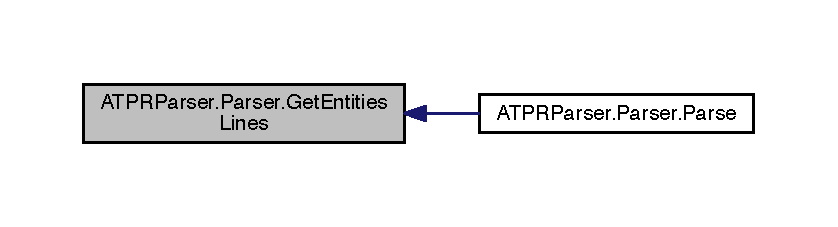
\includegraphics[width=350pt]{df/d53/class_a_t_p_r_parser_1_1_parser_ae5268f6e00d7c5a30a7cb8f463892772_icgraph}
\end{center}
\end{figure}
\hypertarget{class_a_t_p_r_parser_1_1_parser_a853c07acd90bab8533ae613fd05f3057}{}\label{class_a_t_p_r_parser_1_1_parser_a853c07acd90bab8533ae613fd05f3057} 
\index{A\+T\+P\+R\+Parser\+::\+Parser@{A\+T\+P\+R\+Parser\+::\+Parser}!Get\+Matching@{Get\+Matching}}
\index{Get\+Matching@{Get\+Matching}!A\+T\+P\+R\+Parser\+::\+Parser@{A\+T\+P\+R\+Parser\+::\+Parser}}
\subsubsection{\texorpdfstring{Get\+Matching()}{GetMatching()}}
{\footnotesize\ttfamily static List$<$String\mbox{[}$\,$\mbox{]}$>$ A\+T\+P\+R\+Parser.\+Parser.\+Get\+Matching (\begin{DoxyParamCaption}\item[{string}]{matching\+File\+Path,  }\item[{char}]{sep }\end{DoxyParamCaption})\hspace{0.3cm}{\ttfamily [inline]}, {\ttfamily [static]}}



Gets the matchs of the matching\+File. 

\begin{DoxyReturn}{Returns}
The matching.
\end{DoxyReturn}

\begin{DoxyParams}{Parameters}
{\em matching\+File\+Path} & Matching file path.\\
\hline
\end{DoxyParams}
\hypertarget{class_a_t_p_r_parser_1_1_parser_a4d0782c4136575c1b9a33102be225ea1}{}\label{class_a_t_p_r_parser_1_1_parser_a4d0782c4136575c1b9a33102be225ea1} 
\index{A\+T\+P\+R\+Parser\+::\+Parser@{A\+T\+P\+R\+Parser\+::\+Parser}!Parse@{Parse}}
\index{Parse@{Parse}!A\+T\+P\+R\+Parser\+::\+Parser@{A\+T\+P\+R\+Parser\+::\+Parser}}
\subsubsection{\texorpdfstring{Parse()}{Parse()}}
{\footnotesize\ttfamily static List$<$string\mbox{[}$\,$\mbox{]}$>$ A\+T\+P\+R\+Parser.\+Parser.\+Parse (\begin{DoxyParamCaption}\item[{string}]{text,  }\item[{string}]{entity,  }\item[{string}]{orig\+File,  }\item[{string}]{language }\end{DoxyParamCaption})\hspace{0.3cm}{\ttfamily [inline]}, {\ttfamily [static]}}



Parse the document searching for sentences where the entity found. Returns a csv line with the file, the entity the sentence and the sintax analisis of the sentences 


\begin{DoxyParams}{Parameters}
{\em text} & Document text\\
\hline
{\em entity} & Entity.\\
\hline
{\em orig\+File} & Original file.\\
\hline
\end{DoxyParams}
Here is the call graph for this function\+:
\nopagebreak
\begin{figure}[H]
\begin{center}
\leavevmode
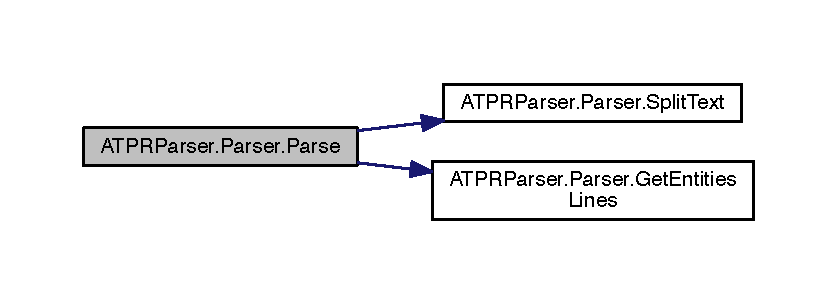
\includegraphics[width=350pt]{df/d53/class_a_t_p_r_parser_1_1_parser_a4d0782c4136575c1b9a33102be225ea1_cgraph}
\end{center}
\end{figure}
\hypertarget{class_a_t_p_r_parser_1_1_parser_adb6ac564b6ddc976a82a46d66f91bb54}{}\label{class_a_t_p_r_parser_1_1_parser_adb6ac564b6ddc976a82a46d66f91bb54} 
\index{A\+T\+P\+R\+Parser\+::\+Parser@{A\+T\+P\+R\+Parser\+::\+Parser}!Split\+Text@{Split\+Text}}
\index{Split\+Text@{Split\+Text}!A\+T\+P\+R\+Parser\+::\+Parser@{A\+T\+P\+R\+Parser\+::\+Parser}}
\subsubsection{\texorpdfstring{Split\+Text()}{SplitText()}}
{\footnotesize\ttfamily static string \mbox{[}$\,$\mbox{]} A\+T\+P\+R\+Parser.\+Parser.\+Split\+Text (\begin{DoxyParamCaption}\item[{string}]{text }\end{DoxyParamCaption})\hspace{0.3cm}{\ttfamily [inline]}, {\ttfamily [static]}}



Splits the text. 

\begin{DoxyReturn}{Returns}
The text.
\end{DoxyReturn}

\begin{DoxyParams}{Parameters}
{\em text} & Text.\\
\hline
\end{DoxyParams}
Here is the caller graph for this function\+:
\nopagebreak
\begin{figure}[H]
\begin{center}
\leavevmode
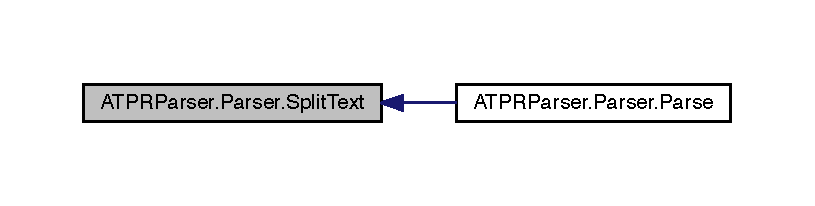
\includegraphics[width=350pt]{df/d53/class_a_t_p_r_parser_1_1_parser_adb6ac564b6ddc976a82a46d66f91bb54_icgraph}
\end{center}
\end{figure}


The documentation for this class was generated from the following file\+:\begin{DoxyCompactItemize}
\item 
A\+T\+P\+R\+P\+A\+R\+S\+E\+R/Parser.\+cs\end{DoxyCompactItemize}

%--- End generated contents ---

% Index
\backmatter
\newpage
\phantomsection
\clearemptydoublepage
\addcontentsline{toc}{chapter}{Index}
\printindex

\end{document}
